\documentclass[border=8pt]{standalone}
\usepackage{fontspec}
\setsansfont{Arial}
\usepackage{pgfplots}
\pgfplotsset{compat=1.18,
  every axis/.append style={/pgf/number format/assume math mode=true,
    tick label style={font=\sffamily\small},
    nodes near coords style={font=\sffamily\scriptsize}}}
% Published-test COCO metrics (%) of the frozen T41 pair.
% Source: docs/t41-results.md, Results table (PR #25).
\begin{document}
\sffamily\small
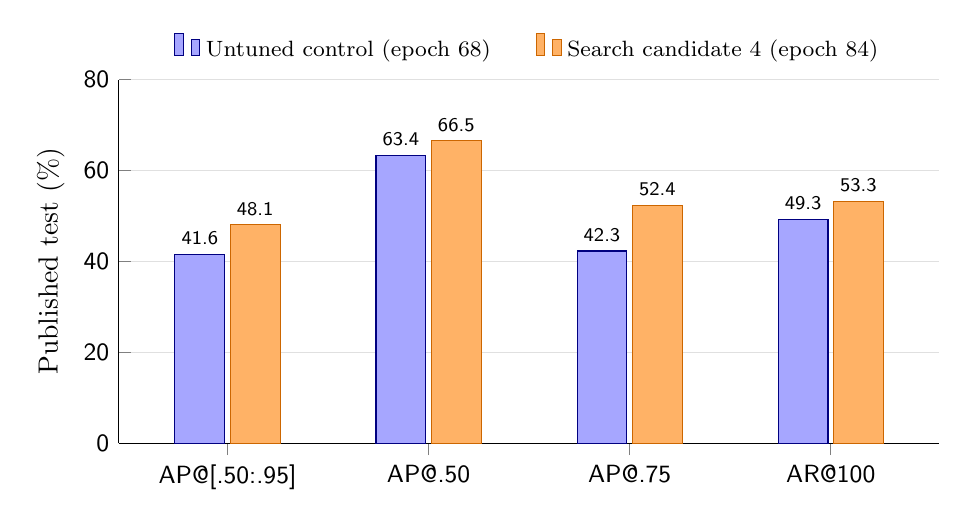
\begin{tikzpicture}
\begin{axis}[
  width=12cm,height=6.2cm,
  ybar,bar width=18pt,
  ymin=0,ymax=80,
  ylabel={Published test (\%)},
  symbolic x coords={AP,AP50,AP75,AR100},
  xticklabels={AP@[.50:.95],AP@.50,AP@.75,AR@100},
  xtick=data,
  enlarge x limits=0.18,
  nodes near coords,
  nodes near coords style={/pgf/number format/.cd,fixed,fixed zerofill,precision=1},
  ymajorgrids,grid style={black!12},
  axis lines*=left,
  legend style={font=\footnotesize,draw=none,fill=none,at={(0.5,1.02)},anchor=south,legend columns=-1,/tikz/every even column/.append style={column sep=0.5cm}},
  legend cell align=left,
]
\addplot[fill=blue!35,draw=blue!50!black] coordinates
  {(AP,41.5886) (AP50,63.4039) (AP75,42.2905) (AR100,49.2603)};
\addplot[fill=orange!60,draw=orange!80!black] coordinates
  {(AP,48.0502) (AP50,66.5397) (AP75,52.3537) (AR100,53.2709)};
\legend{Untuned control (epoch 68),Search candidate 4 (epoch 84)}
\end{axis}
\end{tikzpicture}
\end{document}
